\documentclass[11pt, xcolor=dvipsnames]{beamer}
\usepackage[latin1]{inputenc}
\usepackage[ngerman]{babel}
\usepackage{amsmath}
\usepackage{lmodern} %f�r mathmode wichtig
\usepackage{amsfonts}
\usepackage{amssymb}
\usepackage{graphicx}
\usetheme{Madrid}
\usepackage{textpos}
\usepackage{tikz}
\usepackage[section,boxed]{algorithm}
\usepackage[boxed]{algorithm}
\usepackage{algpseudocode}
\usepackage{caption}
\usepackage{tikz}
\usepackage{subfig}
\usepackage{color}
\usepackage{url}                                            % %url{}-Kommando
\usepackage{fancyhdr,float}                                 % %Kopf-/Fu�zeilen
\usepackage[round]{natbib}                                  % %Zitate
%\usepackage{enumitem}
\usepackage{setspace}
\usepackage[export]{adjustbox} %Rahmen um Bilder
%F�r Pr�sentationsmodus
\usepackage{hyperref}
\hypersetup{pdfpagemode=FullScreen}

\usepackage{multirow}

\usepackage{ dsfont }

%Farbe des Beamer-Themes �ndern
\usecolortheme[named=LimeGreen]{structure}
\makeatletter
\setbeamercolor{frametitle}{fg=black}
\setbeamercolor{title}{fg=black}
\setbeamercolor{palette primary}{fg=black,bg=LimeGreen!30!white} 
\setbeamercolor{palette secondary}{fg=black,bg=LimeGreen!50!white}
\setbeamercolor{palette tertiary}{fg=black,bg=LimeGreen }

\makeatother



%Beschriftung der Fu�leiste der Folien anpassen - Section und Subsectiontitel m�ssen vor jeder Folie (vor \begin{frame}) eingef�gt werden
\makeatletter
\setbeamertemplate{footline}
{
	\leavevmode%
	\hbox{%
		\begin{beamercolorbox}[wd=.333333\paperwidth,ht=4.25ex,dp=1ex,center]{author in head/foot}%
			\vfill
			\vspace{0.9ex}
			\usebeamerfont{author in head/foot}\insertsection
		\end{beamercolorbox}%
		\begin{beamercolorbox}[wd=.333333\paperwidth,ht=3.25ex,dp=1ex,center]{title in head/foot}%
			\vfill
			\vspace{0.4ex}
			\usebeamerfont{title in head/foot}\insertsubsection
		\end{beamercolorbox}%
		\begin{beamercolorbox}[wd=.333333\paperwidth,ht=2.25ex,dp=1ex,right]{date in head/foot}%
			\vfill
			\usebeamerfont{date in head/foot}\inserttitle\hspace*{2em}
			\insertframenumber{} / \inserttotalframenumber\hspace*{2ex} 
		\end{beamercolorbox}}%
	\vskip0pt%
}
\makeatother

\mode<presentation>

\begin{document}

	\author{Antonie Vietor}
	\title{\textbf{Zusatzfolien} \\ K-Means}
	\subtitle{Im Rahmen der Proseminar-Vortragsreihe \\ "Grundlagen des Data-Minings f�r strukturierte Daten" \\ Dr. Nils M. Kriege}
	\date{5. Februar 2018}
	\setbeamercovered{transparent}	
	
	%Ausschalten der Navigationssymbole
	\setbeamertemplate{navigation symbols}{} 
	
	%\logo{logo text} %fuer Logo auf allen Folien
	
	%Logo nur f�r Titelseite
	%\titlegraphic{
	%
\includegraphics[width=5cm]{tud_logo_rgb}
	%\hspace*{6.75cm}~
	%}
	
	%\institute{}
	
	%\subject{}

	

%Titlefolie	
\begin{frame}[plain]
	\maketitle
	%Logo fuer Titelseite mit Positionierung oben links
	\begin{textblock*}{4.5cm}(0cm,-7.75cm)
	
\includegraphics[width=4.5cm]{tud_logo_rgb}
	\end{textblock*}

	%Lehrstuhlbezeichnung mit Positionierung unten links
	\begin{minipage}[b]{7cm}
		\scriptsize
		Fakult�t f�r Informatik\\ 
		Algorithm Engineering (Ls11)\\
		Technische Universit�t Dortmund
	\end{minipage} 

\end{frame}

%Zentrierung der Titel aller Folien
\setbeamertemplate{frametitle}[default][center]

%Folie 2
\section{BFR: Herleitung der Varianz}
\subsection{zu Folie 17}
\begin{frame}
\frametitle{Herleitung der Varianz beim BFR-Algorithmus}
\vspace{-0.55cm}
\begin{columns}[T]
	\begin{column}{0.65\textwidth}
		\begin{flalign*}
			s^2 &= \frac{1}{n} \sum_{i=1}^{n} (x_{i} - \bar{x\:})^2 \\ 
			\visible<2->{
			& =  \frac{1}{n} \sum_{i=1}^{n} (x_{i}^2 - 2x_{i}\bar{x\:}+\bar{x\:}^2) \\}
			\visible<3->{
			& =  \frac{1}{n}\left(  \sum_{i=1}^{n} x_{i}^2 - \textcolor{blue}{\sum_{i=1}^{n} 2x_{i}\bar{x\:}}+\sum_{i=1}^{n} \bar{x\:}^2\right)  \\}
			\visible<10->{
			&= \frac{1}{n}\left(  \sum_{i=1}^{n} x_{i}^2 - \textcolor{blue}{2n \bar{x\:}^2}+ n  \bar{x\:}^2\right)  \\}
			\visible<11->{
			&= \frac{1}{n}\left(  \sum_{i=1}^{n} x_{i}^2 -  n  \bar{x\:}^2\right)  \\}
			\visible<12->{
			&= \frac{1}{n} \sum_{i=1}^{n} x_{i}^2 -   \bar{x\:}^2 }
			\visible<13->{ 
			= \textcolor{red}{\frac{SUMSQ}{N} - \left( \frac{SUM}{N} \right) ^2}}
		\end{flalign*}
	\end{column}
	\begin{column}{0.34\textwidth}
		\color{blue}\begin{flalign*}
		\visible<4->{
		\sum_{i=1}^{n} 2x_{i}\bar{x\:} }
		\visible<5->{
		&= 2\bar{x\:} \sum_{i=1}^{n} x_{i} \\}
		\visible<6->{
		&= 2\bar{x\:} \frac{n}{n} \sum_{i=1}^{n} x_{i} \\}
		\visible<7->{
		&= 2\bar{x\:}\cdot n \cdot \textcolor{red}{ \frac{1}{n} \sum_{i=1}^{n} x_{i} } \\}
		\visible<8->{
		&= 2\:\bar{x\:} n\: \textcolor{red}{\bar{x\:}} \\}
		\visible<9->{
		&= 2n \bar{x\:}^2}
		\end{flalign*}
	\end{column}
\end{columns}


\end{frame}

%Folie 3
\section{Clusterzentrum - Mittelwert}
\subsection{zu Folie 18}
\begin{frame}
	\frametitle{Clusterzentrum als Mittelwert der Datenpunktkoordinaten}
	\begin{block}{}
		Koordinaten des Clusterzentrums entsprechen f�r jede Dimension den Mittelwerten der Datenpunktkoordinaten f�r diese Dimension, also:
			\begin{flalign*}		
				c &= \frac{1}{n} \sum_{i=1}^{n} a_{i} \\
			\visible<2->{
				&= \frac{1}{n} \sum_{i=1}^{n} \left( \begin{array} {c}{a_{i1}}\\{a_{i2}}\end{array}\right)   \\}
			\visible<3->{
				&= \frac{1}{n} \left( \begin{array} {c}{\sum_{i=1}^{n} a_{i1}}\\{\sum_{i=1}^{n} a_{i2}}\end{array}\right)   \\}
			\visible<4->{
				&= \left( \begin{array} {c}{ \overline{a_{1}} }\\{\overline{a_{2}} }\end{array}\right)   \\}
			\visible<5->{
				&= \bar{a\:} }
			\end{flalign*}
	\end{block}
\end{frame}

%Folie 4
\section{$\sum_{i=1}^{n} (a_{i}-\bar{a\:}) = 0$}
\subsection{zu Folie 18}
\begin{frame}
\frametitle{}
	\begin{columns}[T]
		\begin{column}{0.3\textwidth}
			\begin{block}{}
				Gegeben sei:
				\[ a_{i}=\left( \begin{array} {c}{1}\\{2}\\{3}\\{4}\\{5}\end{array} \right)  \]
				\[ \rightarrow \bar{a\:} = 3 \]
			\end{block}
		\end{column}
		\begin{column}{0.6\textwidth}	
			\visible<2->{		
			\begin{block}{}
				{\Large \textcolor{blue}{Es gilt $\sum (a_{i}-\bar{a\:}) = 0$:}}
				\[\sum_{i=1}^{n} (a_{i}-\bar{a\:})  = -2+(-1)+0+1+2 =0\]
			\end{block}}
			\vspace{0.5cm}
			\visible<3->{
			\begin{block}{}
				{\Large \textcolor{blue}{Aber $\sum (a_{i}-\bar{a\:})^2 \neq 0$:}}
				\[\sum_{i=1}^{n} (a_{i}-\bar{a\:})^2  = 4+1+0+1+4 =10\]				
			\end{block}}
		\end{column}
		
	\end{columns}

\end{frame}

%Folie 5
\section{Abstand}
\subsection{zu Folie 5}
\begin{frame}[t]
	\frametitle{Abstand zwischen 2 Punkten}
	%\begin{figure}
		%\vspace{-0.19cm}
		\only<1>{
			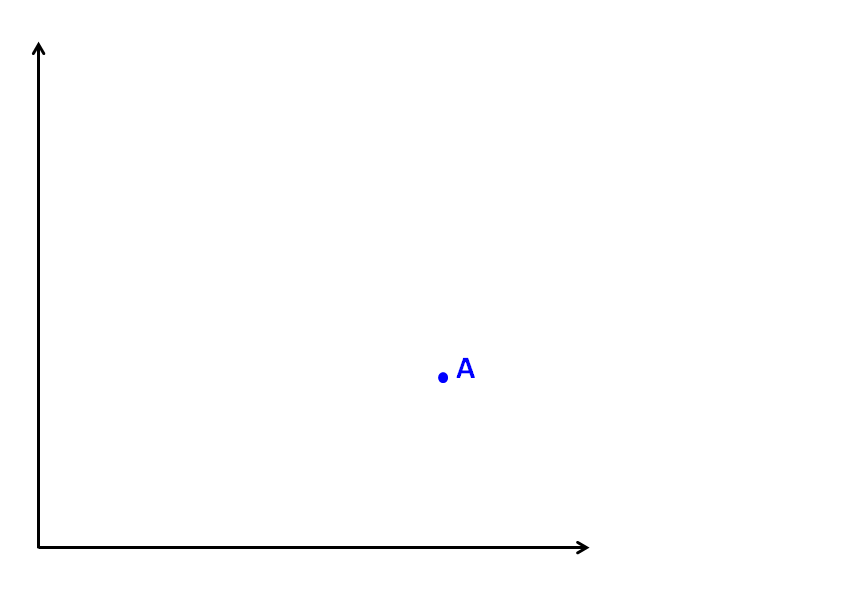
\includegraphics[width=10cm] {1.png} }	
		\only<2>{
			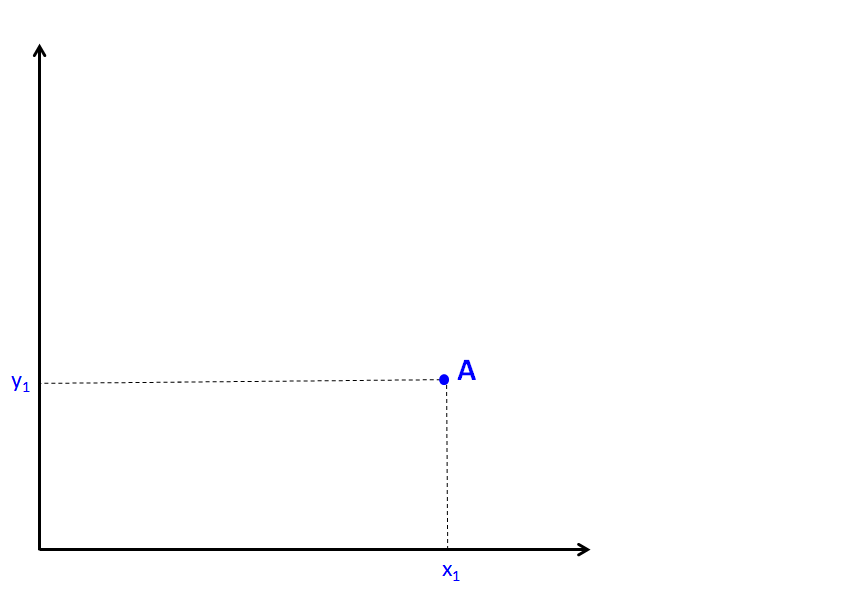
\includegraphics[width=10cm] {2.png} }
		\only<3>{
			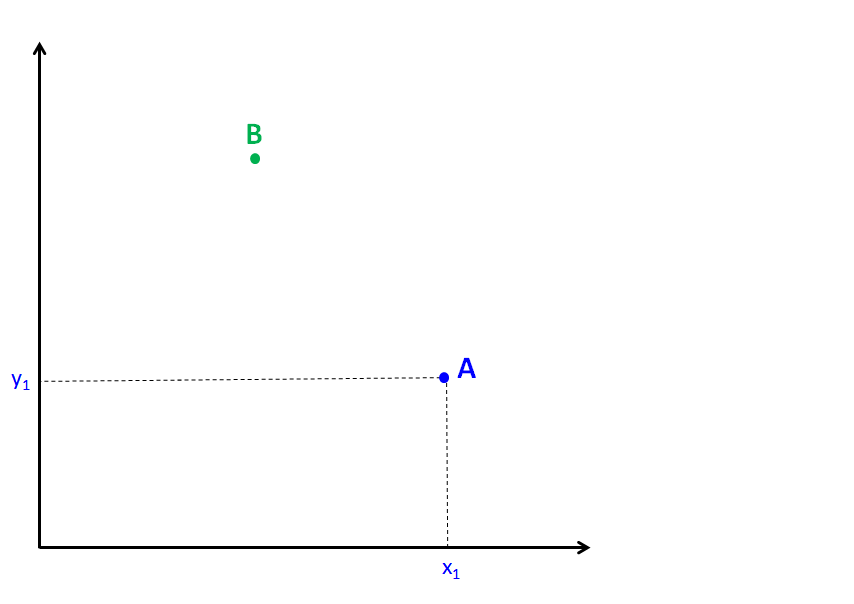
\includegraphics[width=10cm] {3.png} }
		\only<4>{
			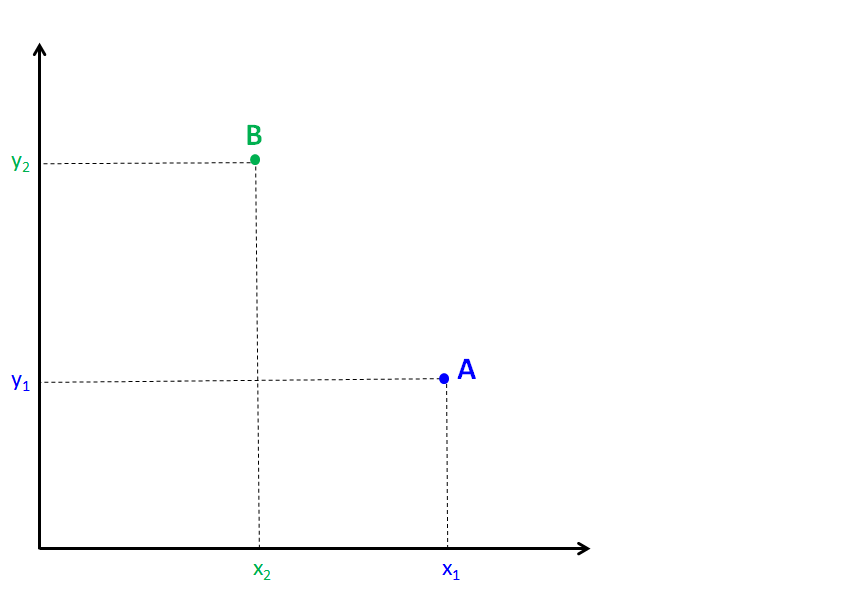
\includegraphics[width=10cm] {4.png} }
		\only<5>{
			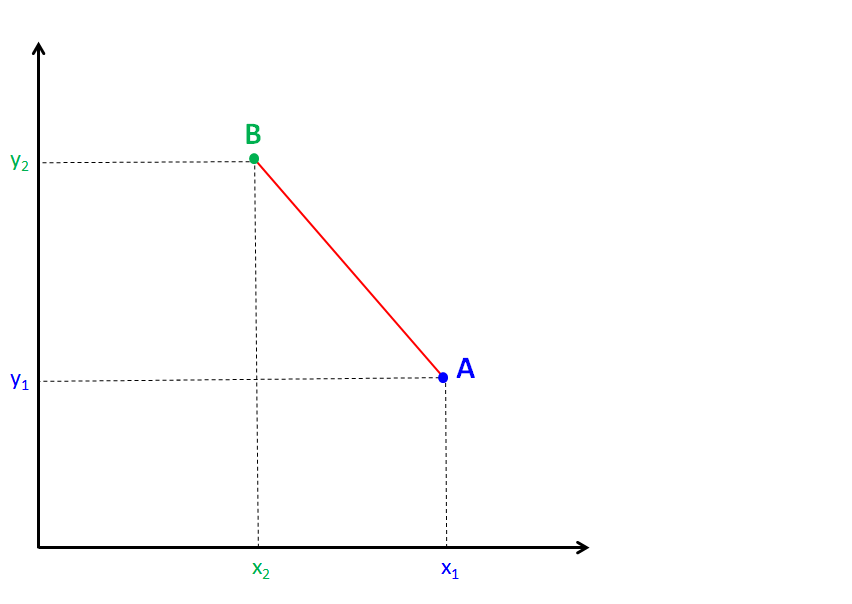
\includegraphics[width=10cm] {5.png} }
		\only<6>{
			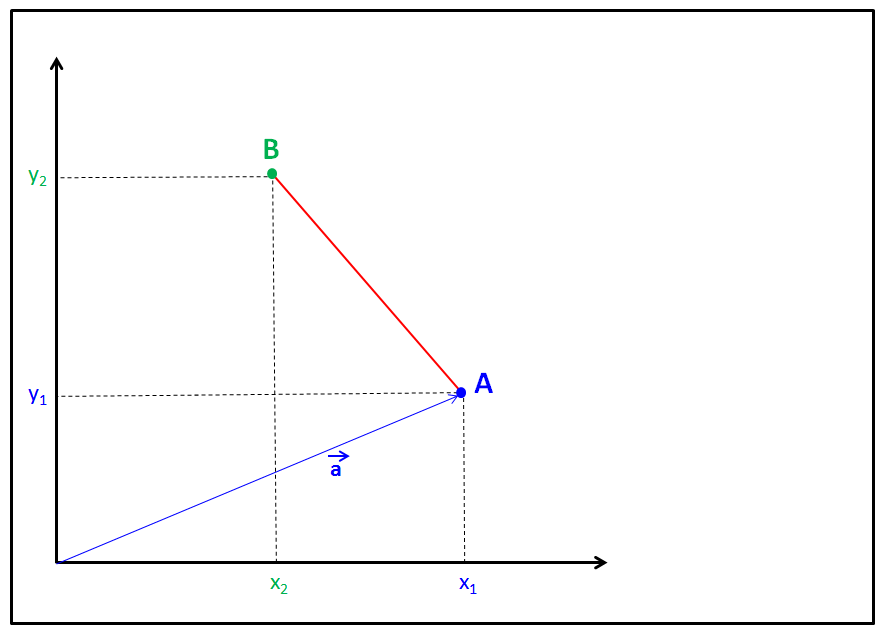
\includegraphics[width=10cm] {6.png} }
		\only<7>{
			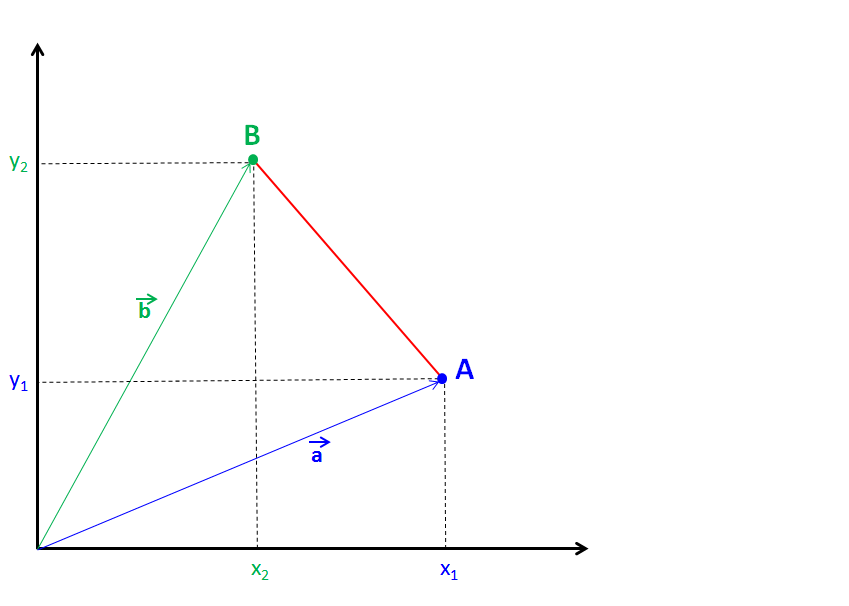
\includegraphics[width=10cm] {7.png} }
		\only<8>{
			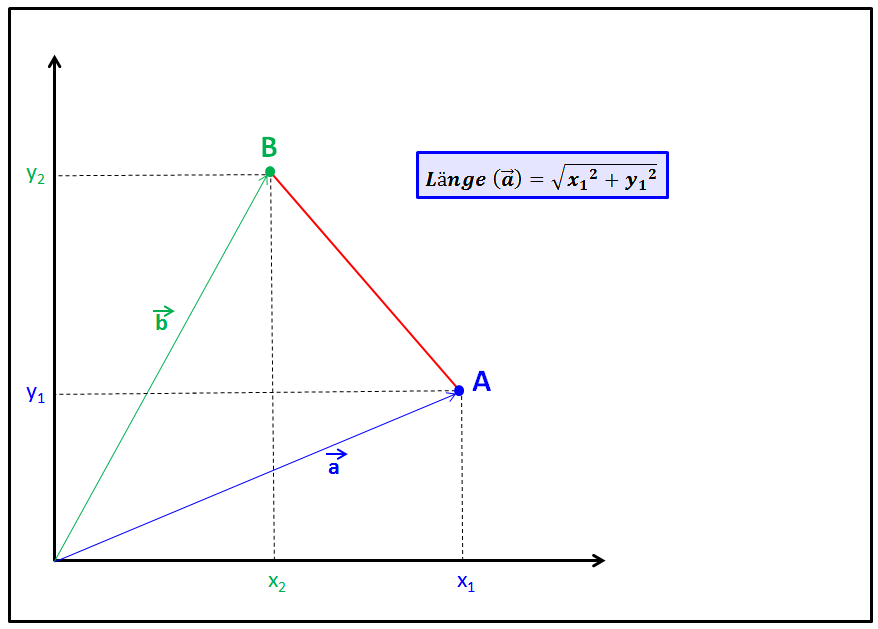
\includegraphics[width=10cm] {8.png} }
		\only<9>{
			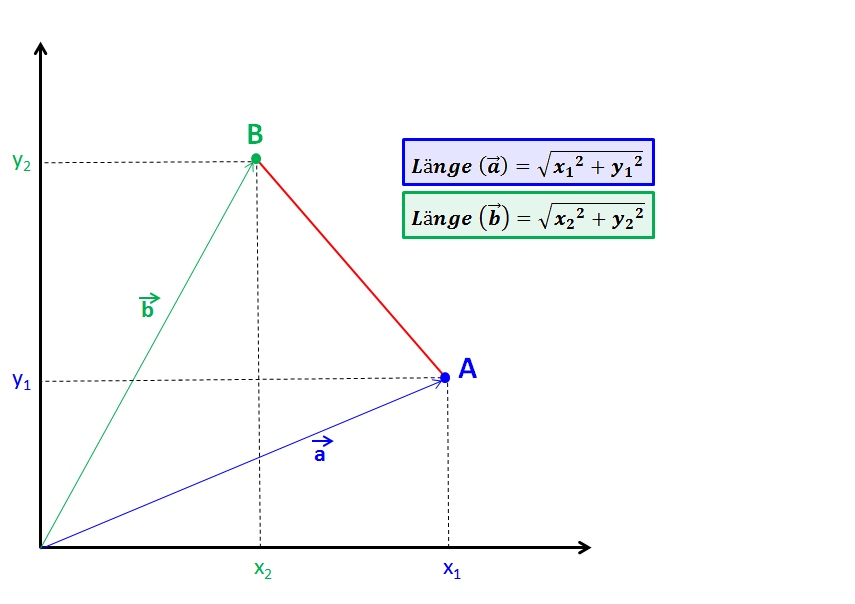
\includegraphics[width=10cm] {9.png} }
		\only<10>{
			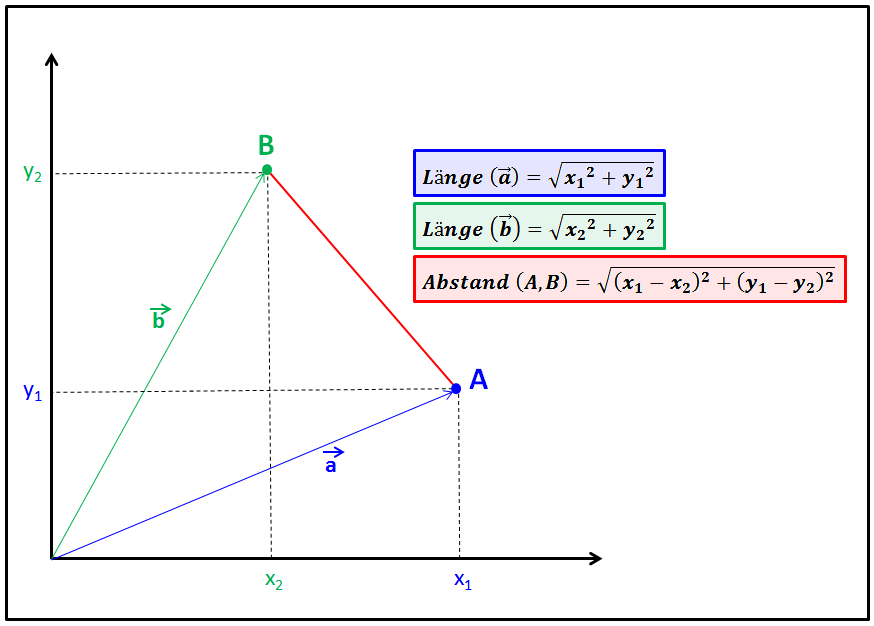
\includegraphics[width=10cm] {10.png} }	
	%\end{figure}
\end{frame}

%Folie 6
\section{Norm}
\subsection{zu Folie 5}
\begin{frame}
	\frametitle{Norm}
	\vspace{0.2cm}
	\begin{definition}[Norm]{
			Sei $ V $ ein Vektorraum �ber $\mathds{K}$. Eine Funktion
			\[V\rightarrow\mathds{R},v\mapsto\|v\|\]
			hei�t Norm auf $V$, wenn sie die nachfolgenden Eigenschaften erf�llt:
			\begin{itemize}
				\visible<2->{
				\item \textbf{Nichtnegativit�t}: F�r alle $v\in V$ gilt $\|v\|\geq0$.}
				\visible<3->{
				\item \textbf{Definiertheit}: F�r alle $v\in V$ gilt $\|v\|=0\Leftrightarrow v=0$.}
				\visible<4->{
				\item \textbf{Homogenit�t}: F�r alle $v\in V$ und alle $\alpha \in \mathds{K}$ gilt $\|\alpha v\| = |\alpha|\|v\|$.}
				\visible<5->{
				\item \textbf{Dreiecksungleichung}: F�r alle $v,w \in V$ gilt $\|v+w\|\leq \|v\| + \|w\|$.}
			
			\end{itemize}
		}
	
	\end{definition}
\vspace{0.2cm}
\visible<6->{Die Norm wird vereinfachend durch $\|\cdot\|$ dargestellt:
	\[\|\cdot\| : V\rightarrow\mathds{R}\]
}
\end{frame}

%Folie 7
\section{$p$-Norm}
\subsection{zu Folie 5}
\begin{frame}
	\frametitle{$p$-Norm}
	\begin{definition}[$p$-Norm]{
		F�r jede nat�rliche Zahl $n \in \mathds{N}$ und jede reelle Zahl $p\geq 1$ definiert man auf dem Vektorraum $\mathds{R}^n$ die sogenannte $ p $-Norm $\| \cdot\|_{p} : \mathds{K}^n \rightarrow \mathds{R}$ durch:	
		\[ \|x\|_{p}:=\left( \sum_{i = 1}^n |x_{i}|^p \right)^\frac{1}{p} = \sqrt[p]{ |x_{1}|^p+|x_{2}|^p+\dots+|x_{n}|^p } \]
		f�r alle $x=(x_{1},x_{2},\dots,x_{n})^T \in \mathds{K}^n$. \\
		\vspace{0.45cm}
		\visible<2->{
		F�r $p=2$ entspricht die $ p $-Norm genau der \textbf{euklidischen Norm} auf $\mathds{R}^n$	
		}}
	\end{definition}
\end{frame}

%Folie 8
\section{Euklidische Norm}
\subsection{zu Folie 5}
\begin{frame}
	\frametitle{Euklidische Norm}
	\begin{definition}[Euklidische Norm]{
		Die euklidische Norm entspricht der Wurzel der Summe der Betragsquadrate der Komponenten des Vektors:	
		\[ \|x\|_{2}:= \sqrt{ \sum_{i = 1}^n |x_{i}|^2}  \]
}		
	\end{definition}
%	\begin{itemize}
%		\item 
%		\item Die Einheitssph�re der reellen euklidischen Norm hat:
%		\begin{itemize}
%		{\normalsize 			
%			\item in 2 Dimensionen die Form ein Kreises
%			\item in 3 Dimensionen die Form einer Kugeloberfl�che
%			\item in allgemeinen Dimensionen die Form einer Sph�re}
%		\end{itemize} 
%	\end{itemize}
\end{frame}

%Folie 9
\section{Euklidische Distanz}
\subsection{zu Folie 5}
\begin{frame}
	\frametitle{Euklidische Distanz}
	\begin{block}{}
		in 2 oder 3 Dimensionen beschreibt die euklidische Norm die L�nge eines Vektors in der Ebene oder im Raum.
		\newline
		F�r p metrische Variablen ist die \textbf{Euklidische Distanz} definiert als:
		\[ \sqrt[p]{ \sum_{i = 1}^n |x_{ik}-x_{ij}|^p} \]
	\end{block}
	\textbf{Definition K-Means von Folie 5}:
	\begin{flalign*}
		J(c_{j}) 
		& = \sum_{a_{i}\in c_{j}}\|a_{i} - c_{j}\|^2 \\
		& = \sum_{a_{i}\in c_{j}} \left( \sqrt{ \sum_{i = 1}^n |a_{i}-c_{j}|^2 }  \right)^2 \\
		& =  \sum_{a_{i}\in c_{j}} |a_{i}-c_{j}|^2  = \sum_{a_{i}\in c_{j}}d^2(a_{i},c_{j}) 
	\end{flalign*}
\end{frame}



\end{document}